\chapter{Marco teórico y estado del arte}
\label{cap:MarcTeorico}

Este capítulo busca realizar una contextualización de los conceptos necesarios para entender el problema que se está tratando por medio de una breve reseña de cada uno, además de a conocer la revisión de los trabajos existentes capaces de realizar tareas similares o basadas en principios similares a los planteados por la solución expuesta de éste trabajo.

\section{Marco teórico}
\label{intro:motivacion:marco}

Se presentan las definiciones de herramientas y técnicas presentados y que sustentan a la solución implementada.

\subsection{Sistemas de procesamiento de \textit{streams}}
\label{subsec:SPS}

El sistema tradicional de procesamiento, el trabajo por lotes (\textit{batch}), está pensado en que primero los datos son recopilados y almacenados, una vez que ésto se ha hecho pasan a ser procesados, pero ¿qué pasa si este enfoque no sirve y los datos han de ser procesados conforme éstos van llegando? 

Para realizar esto es que existe otro enfoque de procesamiento, el procesamiento de \textit{streams}, este enfoque no quita que se puedan almacenar los datos para un análisis \textit{a posteriori}, pero está pensado para trabajar con datos que llegan al sistema directamente desde la fuente y en gran cantidad y son procesados uno por uno.

Un sistema de procesamiento de \textit{streams} se caracteriza, principalmente, por lo siguiente:

\begin{itemize}
\item En memoria: procesamiento contínuo en flujos de datos en series de tiempo.
\item Escalable: arquitectura optimizado para latencia cercana a cero en grandes volúmenes de datos.
\item Escalabilidad a través de la distribución eficiente en múltiples procesadores o servidores.
\end{itemize}

Su funcionamiento es caracterizado por información llegando y es asignada a un nodo, donde sufre alguna transformación al pasar por ellos. 

Conceptualmente su arquitectura es la de una red de elementos ejecutándose de forma concurrente y que operan el flujo de información que va llegando. La Figura \ref{fig:ArqSPS} presenta cómo es una típica arquitectura de éstos sistemas, \cite{SPExplained}.

\begin{figure}[H]
	\centering
	\captionsetup{justification=centering}
	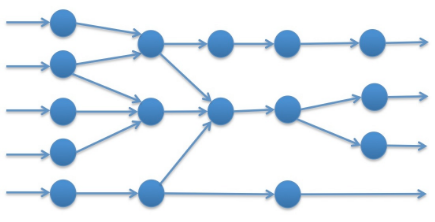
\includegraphics[scale=0.8]{images/ArqSPS.png}
	\caption[Arquitectura típica de sistemas de procesamiento de \textit{streams}.]{Arquitectura típica de sistemas de procesamiento de \textit{streams}.\\Fuente: \cite{SPExplained}}
	\label{fig:ArqSPS}
\end{figure}

Uno de los sistemas de procesamiento de \textit{stream} que ha cobrado relevancia en el último tiempo es \textit{Apache Storm}.

\subsubsection*{Apache Storm}
\label{subsubsec:ApacheStorm}

\textit{Apache Storm} es un sistema que sirve para recuperar \textit{streams} de datos en tiempo real desde una o múltiples fuentes de manera distribuida, tolerante a fallos y en alta disponibilidad. \textit{Storm} está principalmente pensado para trabajar con datos que deben ser analizados en tiempo real, \cite{Storm}.

Es escalable, tolerante a fallos y garantiza que toda la información será procesada. Presenta \textit{Benchmarks} que señalan que por nodo es capaz de procesar más de un millón de tuplas por segundo.

Un sistema construido haciendo uso de \textit{storm} está compuesto por elementos procesadores de dos tipos. El primero es denominada \textit{Spout} y es el encargada de recoger el flujo de datos de entrada. El segundo es denominada \textit{Bolt} y es el encargada de la transformación o procesado de los datos.

Oficialmente, una aplicación \textit{storm} es representada como puede verse en la Figura \ref{fig:stormBeLike}, allí los \textit{Spouts} son representados simulando ser llaves de agua desde donde fluyen los datos al sistema y los \textit{Bolts} como rayos donde se procesa el flujo.

\begin{figure}[H]
	\centering
	\captionsetup{justification=centering}
	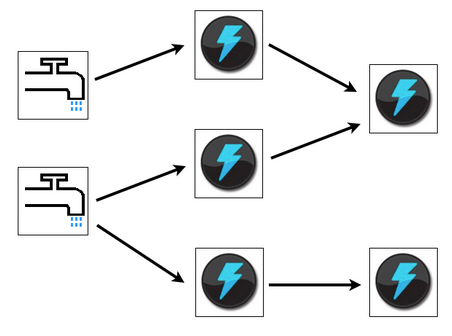
\includegraphics[scale=0.6]{images/stormBeLike.png}
	\caption[Representación del funcionamiento de Apache Storm.]{Representación del funcionamiento de Apache Storm.\\Fuente: \cite{StormFigure}}
	\label{fig:stormBeLike}
\end{figure}

Uno de los puntos fuertes que tiene este sistema, y que está en línea con lo señalado para sistemas de procesamiento de \textit{stream}, es que al crear una topología donde se instancian \textit{Bolts} y \textit{Spouts}, Storm se encarga de escalar el sistema distribuyendo los elementos en sus componentes.

\textit{Spout} y \textit{bolts} se unen para dar origen a una topología. Una topología de Storm es similar a un grafo acíclico dirigido, donde cada nodo se encarga de procesar una determinada información y le pasa el testigo al siguiente nodo. Está compuesta por \textit{Spouts} y \textit{Bolts}, \cite{Storm}.

Se refiere a la forma en la que se van a compartir los datos entre los componentes. Como modelo de datos, Storm utiliza tuplas que son listas de valores con un nombre específico, \cite{Storm}.

\begin{itemize}
\item Shuffle grouping: \textit{storm} decide de forma \textit{round robin} la tarea a la que se va a enviar la tupla, de manera que la distribución sea equivalente entre todos los nodos.
\item Fields grouping: se agrupan los \textit{streams} por un determinado campo de manera que se distribuyen los valores que cumplen una determinada condición a la misma tarea.
\item All grouping: el \textit{stream} pasa por todas las tareas haciendo multicast.
\item Grobal grouping: el \textit{stream} se envía al \textit{bolt} con ID más bajo.
\item None grouping: es un \textit{Shuffle grouping} donde el orden no es importante.
\item Direct grouping: la tarea es la encargada de decidir hacia donde emitir especificando el ID del destinatario.
\item Local grouping: se utiliza el mismo \textit{bolt} si tiene una o más tareas en el mismo proceso.
\end{itemize}

Storm puede funcionar de dos modos: local y \textit{cluster}. El primero es útil para el desarrollo, pues ejecuta toda la topología en una única JVM, por lo que pueden realizarse fácilmente pruebas de integración, depurar código, etcétera. Este modo simula, haciendo uso de \textit{threads}, cada nodo del Cluster, \cite{Storm}.

El modo Cluster es considerado el \"modo de producción\" y es el modo donde el código es distribuido en máquinas diferentes dentro del Cluster.

La arquitectura de Storm se divide en tres componentes:
\begin{itemize}
\item Master Node: ejecuta el demonio llamado Nimbus, el cual es responsable de distribuir el código a través del cluster. Realiza la asignación y monitorización de tareas en las distintas máquinas del cluster.
\item Worker Node: ejecutan el demonio Supervisor, el cual se encarga de recoger y procesar los trabajos asignados en la máquina donde está siendo ejecutado. En caso de fallo de uno \textit{Worker Node}, Nimbus observa esto y redirige el trabajo a otro.
\item Zookeeper: si bien no es un componente propio de Storm, es necesario para su funcionamiento, pues se encarga de coordinar Nimbus y Supervisor, además de mantener sus estados, pues ambos son \textit{stateless}.
\end{itemize}

\subsection{Minería de texto}
\label{subsec:MineriaTexto}

La minería de textos o \textit{text mining} es una rama de la lingüística computacional que trata de obtener información y conocimiento a partir de conjuntos de datos que en principio no tienen un orden o no están dispuestos en origen para transmitir esa informacion, \cite{IvanFernandez}.

Para introducir este concepto es necesario haber pasado primero por entender el concepto de minería de datos o \textit{data mining}.

\subsubsection*{Minería de datos}
\label{subsubsec:dataMining}

Para la minería de datos los datos son la materia prima, ésta se convierte en información que posteriormente es tratada y utilizada para convertirla en conocimiento. Reune áreas como la estadística, inteligencia artificial, bases de datos (la materia prima), y procesamiento masivo. \cite{LuisMolina} la define como \"la integración de un conjunto de áreas que tienen como propósito la identificación de un conocimiento obtenido a partir de las bases de datos que aporten un sesgo hacia la toma de decisión\".

La principal diferencia de la minería de datos con respecto a la minería de textos es que la primera utiliza bases de datos como materia prima, mietras la segunda hace uso de documentos para ello.

Una de las aplicaciones de la minería de textos es la clasificación de documentos. Esta práctica consiste en el uso de técnicas de aprendizaje automático para asignar categorías a un determinado texto, para ello existen algoritmos de clasificación con los cuales pueden construirse clasificadores.

\subsubsection*{Clasificadores}
\label{subsubsec:Classifiers}

En el campo del procesamiento de lenguaje natural el detectar patrones es una parte central. La clasificación es la tarea de seleccionar la etiqueta correcta para una entrada dada. Cada entrada es considerada como aislada de las demás, y el set de etiquetas (o categorías), es definido con anterioridad.

Un clasificador es llamado \"supervisado\" si ha sido construido a partir de un conjunto de datos de entrenamiento o \textit{corpus} de entrenamiento. La Figura \ref{fig:NPLK} muestra el proceso de entrenamiento y uso de un clasificador. (a) Durante el entrenamiento, un estractor de características es utilizado para convertir cada entrada a un conjunto de característica, éstos capturan la información básica de cada conjunto de entrada que es usada para clasificar. Pares de éstos conjuntos y etiquetas son la entrada para el algoritmo que contruye el modelo de clasificación. (b) Durante la predicción se realiza el mismo procedimiento, pero sin entregar como entrada la etiqueta correspondiente, se pasa al modelo generado para obtener las etiquetas predictas.

\begin{figure}[H]
	\centering
	\captionsetup{justification=centering}
	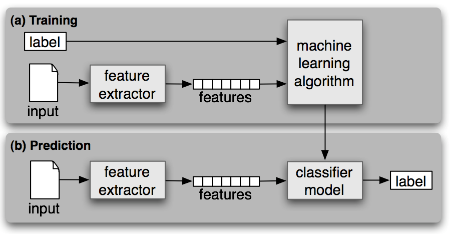
\includegraphics[scale=0.8]{images/TrainingPrediction.png}
	\caption[Clasificación supervisada.]{Clasificación supervisada.\\Fuente: \cite{NPLK}}
	\label{fig:NPLK}
\end{figure}

Para decidir si el modelo de clasificación construido es preciso, éste debe evaluarse. Para ello se ha de tener un conjunto de datos de evaluación. Típicamente corresponde a la misma entrada, donde se evalúa el resultado obtenido por el clasificador con el definido en ésta, separando el conjunto de entrenamiento en dos categorías: los datos de entrenamiento y los datos de evaluación. Comúnmente, se utiliza un 10\% del conjunto total para formar los datos de evaluación.

La métrica más simple para evaluar un clasificador es la precisión (\textit{accuracy}), ésta corresponde al ratio de entradas clasificadas correctamente. Matemáticamente:

\[
	Accuracy = \frac{TP}{TP+FP}
\]

TP y FP corresponden respectivamente a valores correctamente clasificados (\textit{true positives}) y valores clasificados incorrectamente (\textit{false positives}), también conocidos como \"Errores tipo I\". Adicionalmente a éstos existen otros dos: TN y FN que, respectivamente corresponden a valores correctamente no clasificados como elementos de una etiqueta específica (\textit{true negatives}) y los conocidos como \"Errores tipo II\", valores que no pertenecen a una etiqueta y han sido clasificados como tales. Con estos valores se pueden obtener dos nuevas métricas: El \textit{recall} y el medida F (\textit{F-Score}).

El \textit{recall}, indica el ratio de elementos clasificados correctamente y matemáticamente se define como sigue:

\[
	Recall = \frac{TP}{TP+FN}
\]

Por otro lado la Medida F, combina precisión y \textit{recall} para entregar un puntaje. Está dado, en general, dado por la siguiente función:

\[
	F_{\beta} = (1+\beta^{2})\frac{Accuracy · Recall}{(\beta^{2} · Accuracy) + Recall}
\]

Típicamente se utiliza la medida armónica donde $\beta$ toma el valor 1, quedando la función como sigue:

\[
	F1 = 2\frac{Accuracy · Recall}{ Accuracy + Recall}
\]

Se dice que es la medida armónica, pues pondera de igual manera ambos ratios.

Existen diferentes tipos de métodos de aprendizaje de máquina utilizados para construir clasificadores, dentro de ellos existen: \textit{Naïve Bayes}, máxima entropía y árboles de decisión.

En cuanto a los árboles de decisión, éstos corresponden a un diagrama de flujo con el que se decide la etiqueta para una entrada. Los diagramas de flujo consisten en nodos de decisión, los que comprueban los conjuntos de características y las hojas que asignan las etiquetas. El más simple de ellos es llamado un \textit{decision stump}, el cual consiste en sólo un nodo de decisión y múltiples hojas, para construirlo se construye para todas las posibles etiquetas y se calcula la precisión para quedarse con aquellos que alcancen la más alta. Así es como se generaliza, construyendo múltiples \textit{decision stumps} y usando aquelos con más alta probabilidad.

Para el caso de los clasificadores \textit{Naïve Bayes}, \cite{NaiveBayes2}, cada elemento del vector de características aporta en la determinación de qué etiqueta ha de ser utilizada. Para cada etiqueta se calcula su probabilidad \textit{a priori}, utilizando como referencia la frecuencia de ésta en el conjunto de entrenamiento. Esta probabilidad en conjunto con el aporte de cada elemento del vector determina una probabilidad de pertenencia, se le asigna a la entrada la etiqueta que tenga mayor probabilidad de pertenencia.

Para el caso de los clasificadores mñaxima entropía, son similares a los clasificadores bayesianos, pero en lugar de utilizar las probabilidades establecer los parámetros del modelo, utiliza técnicas de búsqueda para encontrar parámetros que maximicen el desempeño del clasificador mediante técnicas de optimización iterativa, las que inician los parámetros en valores aleatoreos y los refina mientras se va acercando al óptimo. Su principal desventaja es que toman mucho tiempo en realizar el aprendizaje por el periodo de iteración antes mencionado, \cite{NPLK}.

\subsection*{MongoDB}
\label{subsubsec:mongoDB}

Base de datos no relacional (NoSQL) de código abierto escrita en C++ y está orientada al trabajo en documentos. Lo anterior quiere decir que, en lugar de guardar los datos en registros, lo hace en documentos y éstos son almacenada en una representación binaria de JSON conocida como BSON.

Una de las diferencias fundamentales con respecto a las bases de datos relacionales es que no es necesario que se siga un esquema; en una misma colección - concepto similar a una tabla en las bases de datos relacionales - pueden tener distintos esquemas.

MongoDB fue creado para brindar escalabilidad, rendimiento y disponibilidad. Puede ser utilizado en un servidor único como en múltiples. Esto se logra dado que MongoDB brinda un elevado rendimiento, tanto para lectura como para escritura, potenciando la computación en memoria.

Las consultas en MongoDB se realizan como si se tratase de Javascript entregando como parámetro un objeto JSON. Por ejemplo, dado el documento presentado en la Figura \ref{fig:MongoJsonExample}, parte de una colección llamada \"Personas\"" en MongoDB:

\begin{figure}[H]
	\centering
	\captionsetup{justification=centering}
	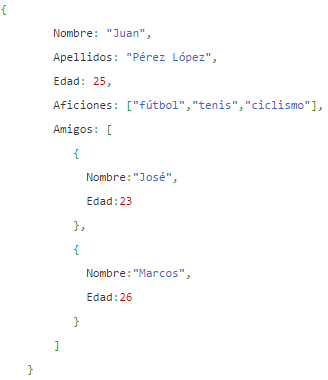
\includegraphics[scale=0.8]{images/MongoJsonExample.png}
	\caption[Ejemplo de representación de un documento en MongoDB.]{Ejemplo de representación de un documento en MongoDB.\\Fuente: Elaboración Propia, (2016)}
	\label{fig:MongoJsonExample}
\end{figure}

Una consulta para encontrar este elemento dentro de la colección se da de la forma aprecida en la Figura \ref{fig:MongoJsonQueryExample}

\begin{figure}[H]
	\centering
	\captionsetup{justification=centering}
	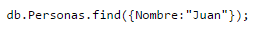
\includegraphics[scale=0.8]{images/MongoJsonQueryExample.png}
	\caption[Ejemplo de consulta en MongoDB.]{Ejemplo de consulta en MongoDB.\\Fuente: Elaboración Propia, (2016)}
	\label{fig:MongoJsonQueryExample}
\end{figure}

En pruebas realizando operaciones habituales dentro de las bases de datos, \cite{MongoPerformance}, demostró que el tiempo de ejecución de MongoDB, como base de datos NoSQL, aventaja significativamente a las bases de datos relacionales más populares como lo son MySQL y PostgreSQL.

\subsubsection*{Play Framework}
\label{subsubsec:playframework}

Es un \textit{framework} de código abierto para aplicaciones \textit{web} escrito en \textit{Java} y \textit{Scala}, el cual sigue el patrón de arquitectura \textit{Modelo-Vista-Controlador} (MVC). Utiliza el paradigma de diseño \"Convención sobre configuración\", el cual apunta a reducir la toma de decisiones que debe tomar el desarrollador sin perder flexibilidad. 

Se enfoca en la productividad, simplificando el desarrollo da aplicaciones mediante procesos automáticos de construcción y despliegue al elimina la desventaja de compilar, empaquetar e implementar el código cuando se realizan cambios, procesos requeridos al utilizar IDEs tradicionales. Los errores son mostrados inmediatamente por medio del navegador. En \textit{Play} por defecto soporta aplicaciones REST y no guarda el estado, permitiendo escalar mediante el uso de múltiples instancias simultaneas, \cite{PlayFramework}.

\subsection*{Mallet}
\label{subsubsec:mallet}

Fué desarrollada por \cite{Mallet}, en la Universidad de Massachusetts Amherst, es una herramienta de Java para el procesamiento de lenguaje natural, clasificación de documentos, \textit{clustering}, extracción de información y otras aplicaciones de aprendizaje de máquina sobre texto.

Cuenta con implementaciones de una variedad de algoritmos entre los cuales se encuentran: \textit{Naïve Bayes}, máxima entropía y árboles de decisión. Además incluye herramientas para evaluar el desempeño de clasificadores mediante el uso de métricas más utilizadas.

\section{Estado del arte}
\label{intro:motivacion:arte}

El problema a abordar consta de dos tópicos centrales: el procesamiento escalable de eventos en tiempo real y clasificación de eventos. Se comienza señalando desde donde inicia este trabajo, seguido de las impresiones de distintos autores respecto al trabajo en redes sociales (\textit{Twitter} específicamente), continuando con sistemas de procesamiento para flujos de información para concluir con la construcción de clasificadores para etiquetado de datos.

\subsection{Plataformas de procesamiento para desastres}
\label{arte:PPDesastres}

El \textit{Qatar Computing Research Institute}, es líder a nivel mundial en la creación de herramientas para dar soporte a desastres naturales usando tecnologías de la información, colaborando con grandes organizaciones como Naciones Unidas, Cruz Roja Internacional y UNICEF. Recientemente, han elaborado distintas aplicaciones (\textit{MicroMappers}, \textit{AIDR}, \textit{UAViators}, etc.), para ayudar a darle sentido al gran flujo de información que reciben los centros de ayuda humanitaria (\textit{Big crisis data}), generada por redes sociales, SMS, imágenes satelitales y aéreas tomadas por drones, que de otra forma serían incapaces de analizar.
Tomando la información, estas aplicaciones unen la ayuda de voluntarios y profesionales digitales, quienes están dispuestos a colaborar a través de internet realizando tareas como identificación o clasificación. Con ésta y el poder del aprendizaje de máquina, se entrenan algoritmos para analizar millones de datos.

\textit{Micromappers} es una aplicación, creada por \textit{Qatar Computing Research Institute}, que permite a voluntarios digitales etiquetar diferente tipos de información para la ayuda en el proceso de respuesta a desastres y desplegarlos en un mapa. En el caso del terremoto de Nepal por ejemplo, los voluntarios han contribuido revisando miles de \textit{tweets} e imágenes para entregar una evaluación de impacto que ayuda a la toma de decisiones. La evolución de esta herramienta está orientada a integrarse con \textit{AIDR} para que la información obtenida de las personas a través de \textit{crowdsourcing} pueda servir para la automatización de proceso de clasificación mediante aprendizaje de máquina, y así subir al análisis de miles a millones de datos generados situaciones de emergencia.

\textit{AIDR} (\textit{Artificial Intelligence for Disaster Response}), \cite{AIDR}, delega al aprendizaje de máquina la identificación de contenido durante desastres en \textit{Twitter}. Va más allá de un simple filtro por palabras clave que limitan la búsqueda a ellas y al lenguaje. Está compuesto de tres partes: El colector, el entrenador y el etiquetador. El primero recolecta y almacena los datos, el entrenador construye un etiquetador automático y permite a usuarios realizar esto dado un conjunto de \textit{tweets} capturados por el colector, el etiquetador analiza los \textit{tweets} clasificados por humanos para automáticamente etiquetar nuevos \textit{tweets}.


\textit{UAViators}, iniciativa también creada por \textit{Qatar Computing Research Institute}, reúne información generada por drones que entregan imágenes para crear conocimiento sobre el área del desastre en tiempo real. Su procesamiento puede entregar información como una estimación de la población afectada, daños en infraestructura de edificios, líneas de electricidad, carreteras, campamentos base, entre otro (http://uaviators.org/).

\subsection{Procesamiento de datos a gran escala}
\label{arte:SPS}

Se presentan a continuación los sistemas de procesamiento de datos a gran escala más utilizados en la actualidad, \cite{PMIProfes}.

\subsubsection*{\textit{MapReduce}}
\label{arte:SPS:mapreduce}

El \textit{framework} de Google \textit{MapReduce}, \cite{DeanMapReduce}, es un modelo de programación diseñado para procesar conjuntos de datos a gran escala en una modalidad orientada al lote (\textit{batch}) o procesamiento \textit{online}. Este sistema esta orientado a programación funcional y utiliza funciones del tipo \textit{map} y \textit{reduce}. \textit{MapReduce} ha logrado gran popularidad en aplicaciones orientadas a grandes volúmenes de datos dado su modelo de programación basado en clave/valor y su escalabilidad. Las soluciones presentadas en  y, \cite{VermaMapReduce}, están orientadas al procesamiento de flujos de datos en línea basadas en \textit{MapReduce}. Los autores en \cite{CondieMapReduce}, proponen modificaciones a \textit{Hadoop}, que es una implementación de \textit{MapReduce} de código abierto, y que permite que los datos sean canalizados entre los operadores haciéndolo mas adecuado a aplicaciones con requerimientos de tiempo real. 

\subsubsection*{Apache S4}
\label{arte:SPS:s4}
					
S4, \cite{NeumeyerS4}, o \textit{Simple Scalable Streaming System}, es un sistema de propósito general, distribuido y escalable que permite que aplicaciones puedan procesar flujos de datos de forma continua y sin restricciones. S4 está inspirado en \textit{MapReduce}, y fue diseñado en el contexto de minería de datos y algoritmos de aprendizaje de máquina en \textit{Yahoo! Labs} para sistemas de publicidad \textit{online}. Cada evento en S4 es descrito como un par (clave, atributo). La unidad básica son los elementos de procesamiento (PEs) y los mensajes que son intercambiados entre ellos. Los PEs pueden emitir o pueden publicar resultados y son alojados en servidores llamados nodos de procesamiento (PNs). Los PNs son responsables de escuchar eventos, rutear eventos a los PEs del nodo y despachar eventos a través de la capa de comunicación. Los eventos son encaminados usando una función de \textit{hashing} sobre los valores de los atributos hacia el PE apropiado. Por otro lado, la capa de comunicación utiliza Zookeeper, \cite{HuntZookeeper}, el cual provee manejo de clusters y reemplazo automático de nodos que fallan. S4 usa encaminamiento estático, es parcialmente tolerante a fallas, y no posee mecanismos de balanceo dinámico de carga.
					
Actualmente S4 está en fase de incubación en la fundación Apache, pero no ha tenido avances en el proyecto desde el año 2013.

\subsubsection*{Apache Storm}
\label{arte:SPS:storm}
					
\textit{Storm} de \textit{Twitter} es una plataforma similar a S4, la cual es publicada como una API para la computación con flujos de datos en tiempo real y de forma escalable. El modelo de programación de Storm está basado en dos primitivas básicas para la transformación de flujos de datos que deben ser implementados de acuerdo a la lógica de las aplicaciones: \textit{spouts} y \textit{bolts}. Un \textit{spout} es una fuente de flujo de datos y un \textit{bolt} hace una transformación de un solo paso sobre el flujo de datos, creando un nuevo flujo basado en la entrada que recibe. Transformaciones complejas requieren múltiples \textit{bolts}, los cuales crean topologías o grafos, el nivel más alto de abstracción en \textit{Storm}. La plataforma soporta tolerancia a fallas a través de un proceso maestro llamado \textit{Nimbus}, el cual garantiza el procesamiento de todos los mensajes a través del uso de una base de datos para el almacenamiento. Sin embargo, esta base de datos es su mayor desventaja respecto de S4 puesto que no es completamente distribuido. Storm define diferentes técnicas para el particionamiento de \textit{streams} de datos y para la paralelización de \textit{bolts}. Sin embargo, se complejiza el desarrollo de aplicaciones. Al igual que S4, Storm usa \textit{Zookeeper} ,\cite{HuntZookeeper}, en la capa de comunicación.

\subsubsection*{Apache Spark}
\label{arte:SPS:spark}

\textit{Spark}, \cite{SparkOnline}, es una plataforma de computación de código abierto para análisis y procesos avanzados, que tiene muchas ventajas sobre \textit{Hadoop}. Desde el principio, \textit{Spark} fue diseñado para soportar en memoria algoritmos iterativos que se pudiesen desarrollar sin escribir un conjunto de resultados cada vez que se procesaba un dato. Esta habilidad para mantener todo en memoria es una técnica de computación de alto rendimiento aplicado al análisis avanzado, la cual permite que \textit{Spark} tenga unas velocidades de procesamiento que sean 100 veces más rápidas que las conseguidas utilizando \textit{MapReduce}. Esta plataforma asegura a los usuarios la consistencia en los resultados a través de distintos tipos de análisis, \cite{Spark}.

\subsection{Escalabilidad de sistema de procesamiento de \textit{streams}}
\label{arte:EscalabilidadSPS}

En los sistemas de procesamiento de \textit{streams}, la escalabilidad puede lograrse usando: (1) paralelización de los elementos de procesamiento y (2) creación y eliminación de nodos de procesamiento. Lo ideal es utilizar ambas técnicas de escalabilidad para lidiar con \textit{stream} masivos de datos que cambian su tamaño en el tiempo.

\begin{itemize}
\item Paralelización: Si el volumen del stream de datos es muy grande, un elemento de procesamiento en una máquina no puede lidiar con el procesamiento, por lo que se requiere paralelizar horizontalmente los operadores. \textit{StreamCloud} \textit{GulisanoStreamCloud} por ejemplo, puede distribuir cualquier elemento de procesamiento en un conjunto de nodos independientes (\textit{share-nothing}). El objetivo es dividir el conjunto de datos en múltiples \textit{sub streams} que fluyen en paralelo. Ésta paralelización es transparente al usuario y se hace en tiempo de compilación. \textit{StreamCloud} agrega un balanceador de carga al inicio de cada división de flujo para redistribuir la salida de los nodos. Además, agrega un agregador de entradas para recibir lo elementos desde los balanceadores de carga. Estos componentes son especializados en el tipo de operador que se quiere paralelizar. Por otro lado, S4 ,\cite{NeumeyerS4}, y \textit{Storm} logran paralelismo horizontal entregándole esta tarea al programador, usando un modelo de programación especialmente diseñado para distribuir elementos de procesamiento. En \textit{Storm}, el \textit{stream} de datos se distribuye equitativamente entre los trabajadores disponibles y en S4 se distribuye generalmente usando una función de \textit{hash} para que los eventos con un mismo valor sean procesados por el mismo elemento de procesamiento.
\item Elasticidad: En el contexto de \textit{cloud computing}, hay un costo asociado al uso de máquinas que no están siendo utilizadas. Por otro lado, si se tiene menos capacidad de la necesaria para el procesamiento se produce sobrecarga de los nodos lo que conlleva la pérdida de datos afectando el rendimiento. Es por eso que agregar y eliminar máquinas en tiempo de ejecución para ajustarse al procesamiento es de suma importancia. En Esc, \cite{SatzgerESC}, para lograrlo existe un módulo administrador que es responsable de mantener estadísticas sobre la carga de las máquinas y el tamaño de los buffers. Esta información es usada para la adaptabilidad y distribución tomando en cuenta los costos monetarios. La función de \textit{hash} se reemplaza con nuevos parámetros para lograr la nueva distribución. Esc introduce el concepto de reescritura del grafo, donde un PE puede dividir y agregar en otros PE.
Similarmente, \textit{TimeStream}, \cite{QianTimeStream}, propone usar una substitución resiliente de cada PE, usando el particionamiento del hash, paralelización de los PE y unión del procesamiento.
SEEP, \cite{CastroFernandezISFT}, por otro lado, tiene un mecanismo para aumentar el número de nodos, detectando cuellos de botella, compartiendo la carga del operador entre un conjunto de nuevos operadores particionados. El estado de la partición se mantiene y se reparticiona el espacio de claves de las tuplas procesadas. Finalmente, \cite{GedikESDSP}, propone auto-paralelizar en tiempo de ejecución. usando migración de estado y monitoreo del flujo de datos.
\item Localización: Otros trabajo se enfocan en optimizar la localización de elementos de procesamiento en los nodos de procesamiento, como el trabajo realizado en el contexto del proyecto FONDEF Idea y T-Storm, \cite{XuTStorm}, que modifica \textit{Storm} de modo de disminuir al máximo el tráfico entre nodos de procesamiento.
\end{itemize}

\subsection{Tolerancia a fallas en sistema de procesamiento de \textit{streams}}
\label{arte:ToleranciaFallasSPS}

Se puede analizar la tolerancia a fallas a nivel de recuperación de nodos de procesamiento caídos o a nivel de procesamiento de \textit{stream}. A nivel del procesamiento de \textit{stream} hay sistemas que proveen la seguridad que una tupla se va a procesar exactamente una vez como \textit{Storm} y otros como S4 \cite{NeumeyerS4} son adecuados en escenarios donde perder una tupla no tiene mayor impacto en el resultado.

\begin{itemize}
\item En los esquemas basados en replicación \cite{HwangTolerancia}, \cite{ShahTolerance} y \cite{BalazinskaTolerance}, el sistema de procesamiento de stream crea un número de copias o réplicas que le permiten tolerar un número igual de fallas simultáneas. En el caso de que una falla ocurra, el operador involucrado es reemplazado por una de sus réplicas la cual posee el mismo estado que el operador fallado. Por otro lado, las técnicas basadas en replicación son capaces de reducir el costo de almacenamiento, sin embargo introducen un alto costo en términos de memoria puesto que deben mantener más recursos de procesamientos sumados a la mantención de la réplica.
\item \textit{Checkpointing}: En los esquemas basados en \textit{checkpoint} \cite{HwangTolerancia}, \cite{WangTolerance1}, cada recurso de procesamiento o operador puede llevar a cabo dos acciones: 1) almacenar periódicamente su estado o 2) retener las tuplas de salida en un \textit{buffer} hasta que estas han sido almacenadas en el siguiente operador. En el caso de que exista una falla, el operador es reiniciado y se le copia el último estado almacenado o checkpoint. S4, \cite{NeumeyerS4}, usa un sistema de archivos para implementar almacenamiento de \textit{checkpointing}. El \textit{checkpointing} puede ser seguido de re-procesar eventos desde el \textit{checkpointing}, sin embargo, puede ser que la complejidad del procesamiento, la masividad de los datos y sobrecarga no lo permita y se requieran aumentar el número de nodos de procesamiento. CEC, \cite{SebepouCEC}, propone un mecanismo que garantiza tolerancia a fallas al tomar \textit{checkpointing} del estado de los PE de manera incremental, entre \textit{checkpoints} se mantiene un \textit{log} de las tuplas en un \textit{buffer}, el cual puede ser restrictivo. \textit{TimeStream}, \cite{QianTimeStream}, al igual que \textit{Storm} y \textit{MillWheel}, \cite{AkidauMillWheel}, provee garantías que las tuplas serán procesadas exactamente una vez, al almacenar estados y las dependencias de salida de cada operador. \textit{Zaharia}, \cite{ZahariaDiscretized}, usa técnicas de procesamiento de batch para mantener la tolerancia a fallas de manera asíncrona y en paralelo, al igual que en SEEP, \cite{CastroFernandezISFT}, donde cada operador es tratado como una entidad independiente.
\item Monitoreo: En Esc, \cite{SatzgerESC}, se utilizan árboles de supervisión de los procesos, donde el padre monitorea a los hijos y los reinicia cuando fallan. El monitoreo se realiza usando mensajes. Otros sistemas confían en sistemas como \textit{Zookeeper} para mantener la tolerancia a fallas del sistema y reemplazar nodos caídos por otros que realicen el procesamiento.
\end{itemize}

\subsection{Clasificación de eventos}
\label{intro:ea:clasificacion}

Por otra parte, la clasificación de texto en servicios de \textit{microblogging}, como \textit{Twitter} es un problema cuya solución tiene diferentes puntos de vista, los métodos tradicionales incluyen hacer uso de una bolsa de palabras para clasificar según el contenido del texto, construcción de n-gramas para clasificar según términos co-ocurrentes o ubicar el texto en una categoría haciendo uso de técnicas de aprendizaje de máquina o \textit{Machine Learning}, \cite{EventDetection}. 
Este último método ya ha sido comprobado por diversos autores, entre ellos \cite{Maldonado}, quien utilizó este método para realizar su memoria donde clasificaba \textit{tweets} según sentimientos positivos, negativos o neutros. 

En el marco de las jornadas chilenas de la computación \cite{WladdimiroPMI}, propusieron un modelo, desarrollado para el proyecto PMI USA 1204: Despliegue agil de aplicaciones para desastres \cite{PMIProfes}, donde analizaron el rendimiento de una aplicación de clasificación de necesidades básica al ser implementada en un sistema de procesamiento de \textit{streams} como S4. En se propone un modelo basado en \textit{Yahoo! S4} donde haciendo uso del paradigma de procesamiento de \textit{streams} de datos se forma un grafo cuyos nodos (Elementos de procesamiento o PE, por sus siglas en inglés), dividen el procesamiento en pequeñas tareas fácilmente replicables para paralelizar el \textit{pepeline}. En esa ocación desarrollaron distintos tipos de operadores mencionados a continuación:

\begin{itemize}
\item Recolector: haciedo uso de la API de \textit{Twitter} obtiene el \textit{stream} de datos del mismo. 
\item \textit{Scheduler}: discrimina cada \textit{tweet} según la categoría que pertenece (Información, agua, electricidad o alimento), mediante el uso de una bolsa de palabras y la distancia \textit{Hamming}.
\item Filtrado: utilizaron en su trabajo un clasificador basado en \textit{machine learning} para verificar la subjetividad de un \textit{tweet}, por lo que ya esta demostrado que esta herramienta es capaz de categorizar texto, por lo que puede ser aplicada para las entradas de \textit{Twitter}.
\item Relevancia: identificar si una información es o no confiable haciendo uso de la cantidad de publicaciones del usuario, sus seguidores y a quienes sigue para estimar una reputación del autor.
\item Ranking: hace uso de la información anterior, decidiendo a qué le entrega mayor importancia.
\end{itemize}

Los autores concluyeron basándose en la carga computacional la importancia de una replicación adecuada para distribuirla entre los PE, pero no fueron concluyentes en cuánto o qué nivel de replicación es el adecuado o cuándo replicar.

A modo de comentario, diversos autores, entre los que podemos mencionar a \cite{VanDeVoort}, \cite{EventDetectionInTwitter}, \cite{Maldonado}, han señalado las dificultades que se presentan al trabajar utilizando como entradas los estados públicos (\textit{tweet}) de los usuarios de \textit{Twitter}, dentro de las dificultades señaladas se encuentran, por ejemplo, el acceso a la información; si bien existen accesos públicos a la información éstos son restringidos tanto en cantidad como en tiempo: Este punto de acceso permite acceder a un 1\% de la información generada en un instante, es decir, por cada cien \textit{tweets} sólo puede accederse a uno de ellos. Sólo se permite realizar 180 consultas cada quince minutos (aproximadamente 12 consultas por minuto) y, en el caso de ser un usuario identificado, se aumenta a 450 consultas dentro del mismo intervalo de tiempo (aproximadamente 30 consultas por minuto). Por otro lado existe un punto de acceso pagado denominado \textit{FireHose} el cual entrega libre acceso a la información.

Por otro lado \cite{VanDeVoort}, señalan que la dificultad radica en el hecho de que cualquier persona puede realizar publicaciones en esta red social, induciendo ruido en la información (considerando el ruido como toda información que aparece junto a la deseada, pero no aporta nueva), además de, al ser publicaciones de máximo 140 caracteres es complejo contextualizar el contenido.
